% ===========================================================================
% Section 4.1.8: Stylized Facts of Accumulation, Distribution, and External Constraints
% Manuscript Module for Chapter 2
% Drafted for inclusion in paper_tex_3.0/section4.tex
% ===========================================================================

\subsection{Stylized Facts of Accumulation, Distribution, and External Constraints}

\paragraph{A}
Before deploying cointegration estimators and state-dependent non-linear specifications, this subsection establishes empirical stylized facts for the United States (1931--2024) and Chile (1940--2010). These visual patterns ground the econometric strategy by demonstrating: (1) long-run co-movement between output and capital stocks (motivating cointegration); (2) multi-decadal decline in output--capital ratios (motivating an aggregate elastic transformation parameter $\theta < 1$); (3) asymmetry between short-run utilization volatility and smooth capital accumulation; and (4) discrete regime shifts in distributive state variables and foreign exchange bottleneck indices.

\subsubsection{Stylized Facts of the U.S. Non-Financial Corporate Economy (1931--2024)}

\paragraph{B}
Figure~\ref{fig:us_stylized_1_y_kcap} displays the empirical trajectories of log real non-financial corporate (NFC) output ($y_t$) and core productive capital stock ($k_t^{cap} = k_t^{\text{ME}} + k_t^{\text{NRC}}$) in Panel A, alongside the log output--capital ratio ($y_t - k_t^{cap}$) in Panel B. Over the 94-year sample, output and core capital drift together along a clear upward historical trend, exhibiting persistent non-stationary behavior. This common drift provides the initial visual justification for searching for a cointegrating relationship $y_t = \alpha + \beta_k k_t^{cap} + \boldsymbol{\beta}'\mathbf{X}_t + u_t$ rather than estimating regressions in stationary first differences.

\FloatBarrier
\begin{figure}[H]
\centering
\caption{U.S. Log Real NFC Output, Core Capital Stock, and Output--Capital Ratio (1931--2024)}
\label{fig:us_stylized_1_y_kcap}
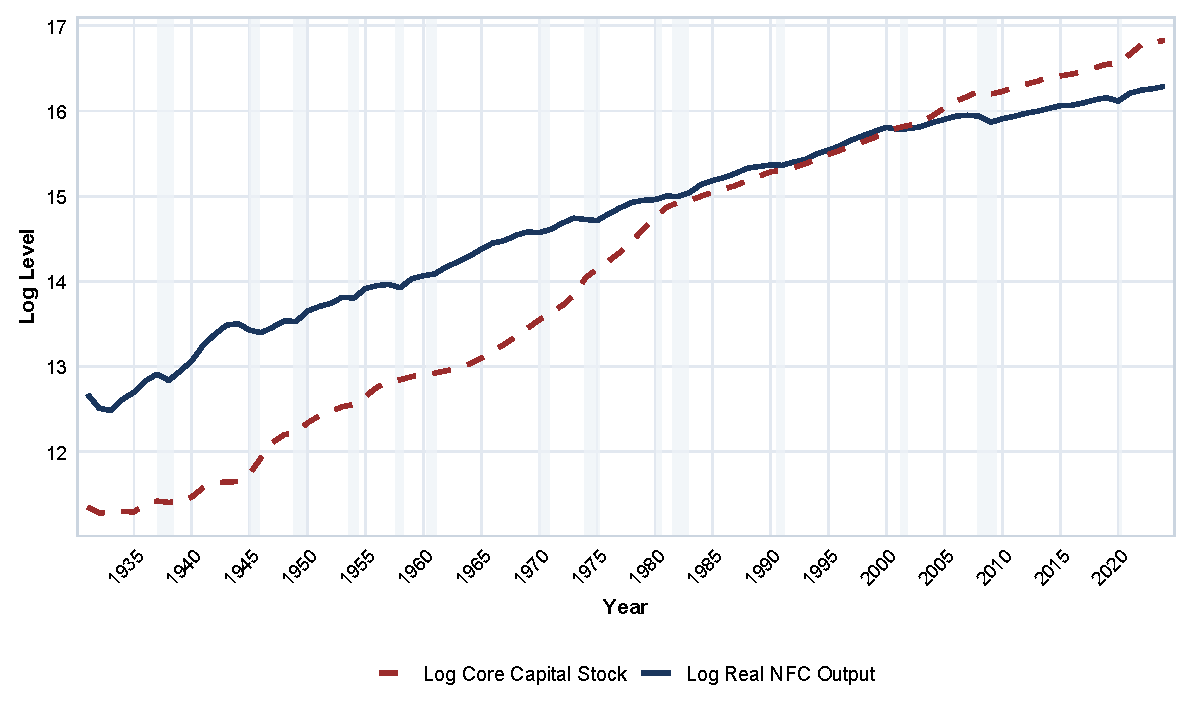
\includegraphics[width=0.92\textwidth]{figures/fig_us_stylized_1_y_kcap.pdf}
\begin{singlespace}\vspace{1ex}
\multicolumn{1}{p{14.5cm}}{\footnotesize \textbf{Note:} Panel A plots log real non-financial corporate gross value added ($y_t$, solid navy line) and log core capital stock ($k_t^{cap} = k_t^{\text{ME}} + k_t^{\text{NRC}}$, dashed crimson line). Panel B plots the log output--capital ratio $y_t - k_t^{cap}$ with a non-parametric LOESS secular trend (dashed amber line). Light gray shaded bands denote official NBER recession dates. Data sourced from BEA NIPA Tables and Fixed Assets Accounts.}
\end{singlespace}
\end{figure}
\FloatBarrier

\paragraph{C}
Crucially, Panel B of Figure~\ref{fig:us_stylized_1_y_kcap} and Figure~\ref{fig:us_stylized_2_yk_ratio} demonstrate that the empirical output--capital ratio ($Y_t / K_t^{cap}$) is not a constant Kaldorian benchmark. Instead, it displays a multi-decadal wave structure: rising during the post-WWII Fordist golden age, peaking in 1966, and entering a persistent secular decline thereafter. This secular downward trajectory falsifies the standard assumption of Harrod-neutral technical progress ($\theta = 1.00$) and confirms that capital accumulation systematically outpaced output capacity expansion over the late twentieth century, visually establishing the empirical plausibility of $\theta < 1$.

\FloatBarrier
\begin{figure}[H]
\centering
\caption{Secular Wave and LOESS Trend of the U.S. Output--Capital Ratio ($Y_t / K_t^{cap}$)}
\label{fig:us_stylized_2_yk_ratio}
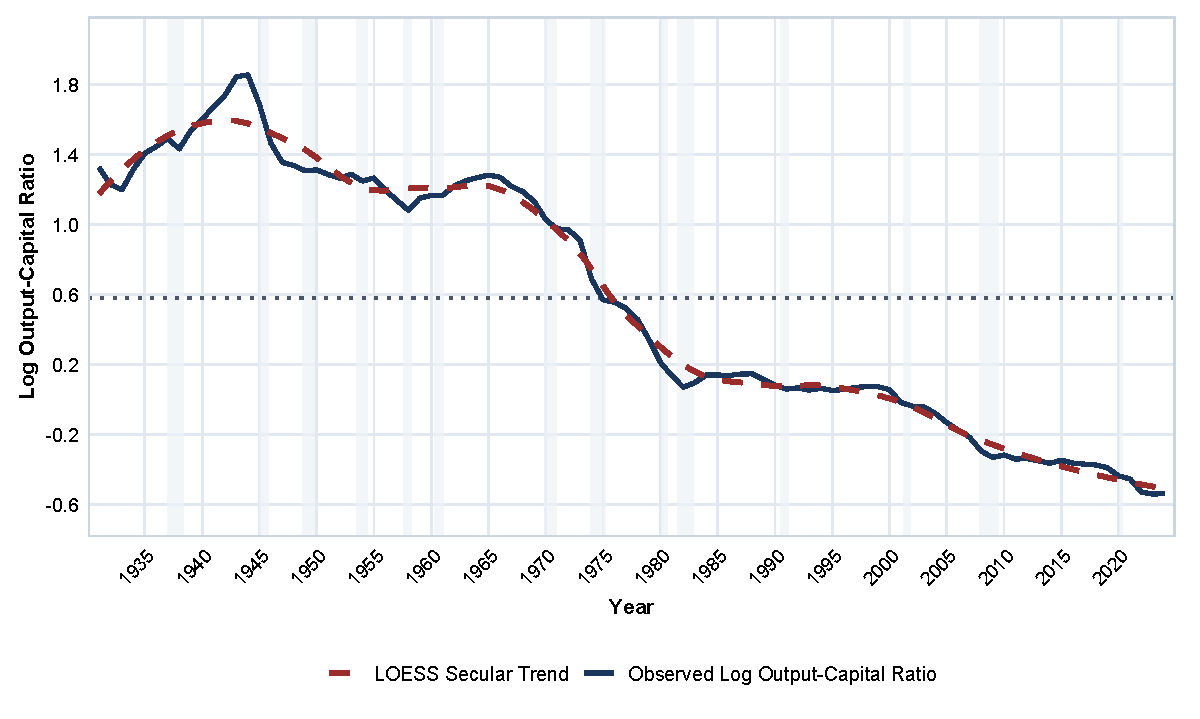
\includegraphics[width=0.92\textwidth]{figures/fig_us_stylized_2_yk_ratio.pdf}
\begin{singlespace}\vspace{1ex}
\multicolumn{1}{p{14.5cm}}{\footnotesize \textbf{Note:} Annual level of output--capital ratio $Y_t / K_t^{cap}$ (solid navy line) relative to full-sample mean baseline (dotted line) and LOESS non-parametric secular trend (dashed crimson line, span = 0.35). Light gray background bands indicate NBER recessions.}
\end{singlespace}
\end{figure}
\FloatBarrier

\paragraph{D}
Figure~\ref{fig:us_stylized_3_growth_rates} contrasts the annual log growth rate of output ($\Delta y_t$) with the annual growth rate of core capital stock ($\Delta k_t^{cap}$). The output growth rate exhibits severe cyclical volatility ($\text{SD} = 0.058$), responding dynamically to short-run effective demand shocks and NBER recessions. In contrast, capital accumulation growth is smooth and persistent ($\text{SD} = 0.019$). This fundamental asymmetry underscores that capacity utilization ($\mu_t = Y_t / Y_t^p$) acts as the primary buffer absorbing effective demand shocks in the short-to-medium run, while potential output ($Y_t^p$) follows the slower structural evolution of capital accumulation.

\FloatBarrier
\begin{figure}[H]
\centering
\caption{Annual Growth Rates of U.S. NFC Output ($\Delta y_t$) vs. Core Capital Stock ($\Delta k_t^{cap}$)}
\label{fig:us_stylized_3_growth_rates}
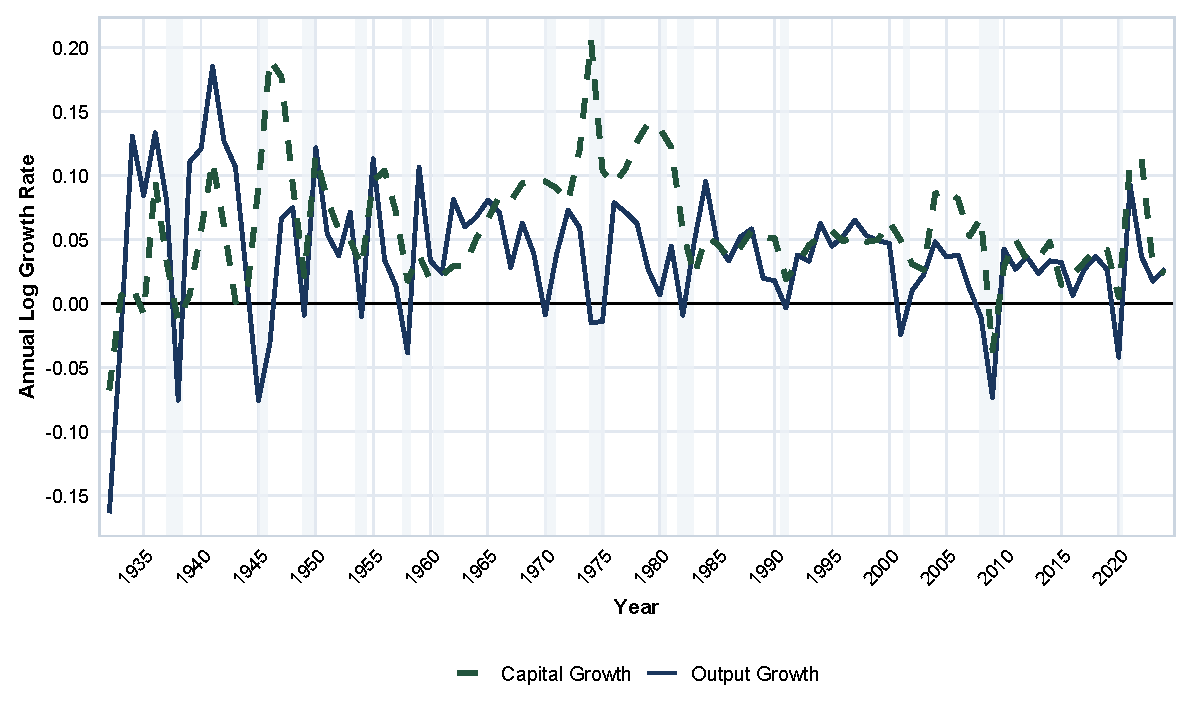
\includegraphics[width=0.92\textwidth]{figures/fig_us_stylized_3_growth_rates.pdf}
\begin{singlespace}\vspace{1ex}
\multicolumn{1}{p{14.5cm}}{\footnotesize \textbf{Note:} Annual log difference of output $\Delta y_t$ (solid navy line) versus core capital accumulation growth $\Delta k_t^{cap}$ (dashed green line). Zero-growth horizontal baseline provided for visual reference.}
\end{singlespace}
\end{figure}
\FloatBarrier

\paragraph{E}
Figure~\ref{fig:us_stylized_4a_distributive_state} and Figure~\ref{fig:us_stylized_4b_distributive_state} track the U.S. distributive and structural state variables that condition the transformation elasticity. Figure~\ref{fig:us_stylized_4a_distributive_state} uses a dual Y-axis plot to contrast the net corporate wage share ($\omega_{t-1}$, left axis, solid navy line) with the Intellectual Property Products (IPP) capital share ($\iota_{t-1} = K_{\text{IPP}} / [K_{\text{cap}} + K_{\text{IPP}}]$, right axis, dashed crimson line). Note on series continuity: Tier 1 net wage share ($\omega_{\text{ST,Tier1}, t-1}$) is plotted here because it provides full-sample coverage (1931--2024), whereas Tier 2 ($\omega_{\text{ST,Tier2}, t-1}$) only begins in 1948 due to BEA supervisory worker data constraints.

\FloatBarrier
\begin{figure}[H]
\centering
\caption{U.S. Net Wage Share ($\omega_{t-1}$) and IPP Capital Share ($\iota_{t-1}$)}
\label{fig:us_stylized_4a_distributive_state}
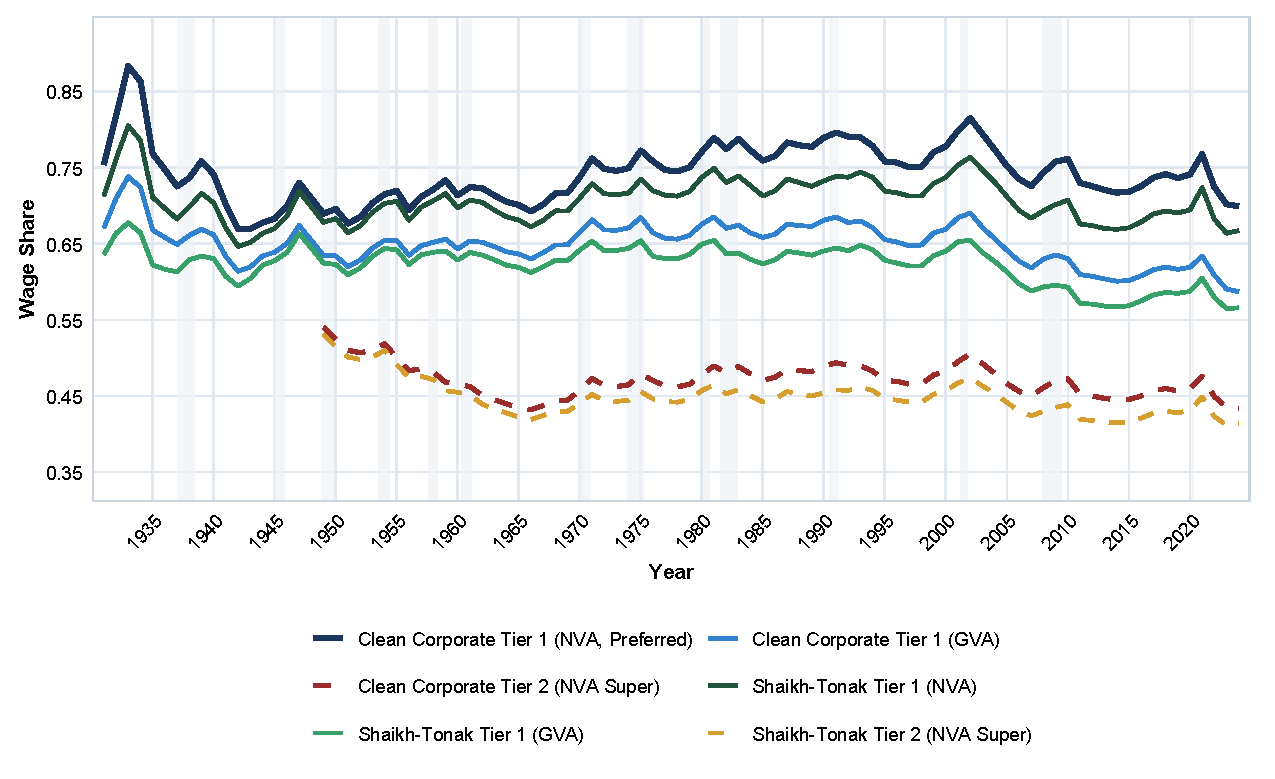
\includegraphics[width=0.92\textwidth]{figures/fig_us_stylized_4a_distributive_state.pdf}
\begin{singlespace}\vspace{1ex}
\multicolumn{1}{p{14.5cm}}{\footnotesize \textbf{Note:} Dual Y-axis plot displaying net corporate wage share $\omega_{t-1}$ on the left axis (solid navy line, Tier 1 full-sample series 1931--2024) and IPP capital share $\iota_{t-1}$ on the right axis (dashed crimson line). Light gray shaded background bands indicate official NBER recessions.}
\end{singlespace}
\end{figure}
\FloatBarrier

\paragraph{F}
Figure~\ref{fig:us_stylized_4b_distributive_state} plots Effective Wage Pressure $C_t = \omega_{t-1}(1 - \iota_{t-1})$. The trajectory reveals distinct institutional periodization: high effective wage pressure during the Fordist accord (1945--1973), followed by structural wage suppression and rising IPP capital intensity during the neoliberal restructuring period (1980--2024). This structural regime behavior motivates incorporating the state-dependent interaction term $k_t^{cap} \times C_t$ in Specification A and B.

\FloatBarrier
\begin{figure}[H]
\centering
\caption{U.S. Effective Wage Pressure Index ($C_t = \omega_{t-1}(1 - \iota_{t-1})$)}
\label{fig:us_stylized_4b_distributive_state}
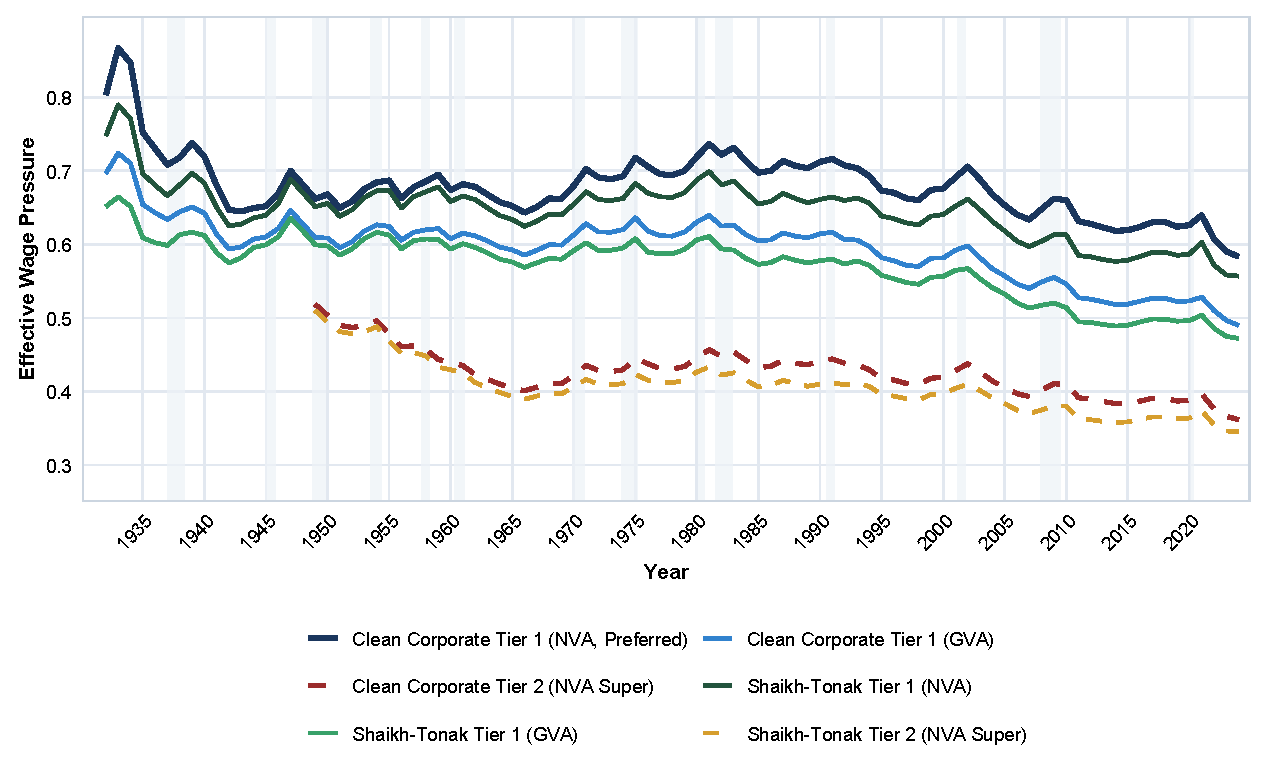
\includegraphics[width=0.92\textwidth]{figures/fig_us_stylized_4b_distributive_state.pdf}
\begin{singlespace}\vspace{1ex}
\multicolumn{1}{p{14.5cm}}{\footnotesize \textbf{Note:} Effective Wage Pressure index $C_t = \omega_{t-1}(1 - \iota_{t-1})$ (solid green line) alongside a LOESS non-parametric secular trend (dashed amber line). Light gray background bands indicate NBER recessions.}
\end{singlespace}
\end{figure}
\FloatBarrier

\begin{table}[H]
\centering
\caption{United States Macroeconomic and Distributive Summary Statistics (1931--2024)}
\label{tab:us_stylized_facts_summary}
\begin{tabular}{p{7.5cm} p{2.5cm} p{2.5cm}}
\hline\hline
\textbf{Variable} & \textbf{Mean} & \textbf{Std. Dev.} \\
\hline
Log Real Output ($y_t$) & 14.734 & 1.107 \\
Log Core Capital Stock ($k_t^{cap}$) & 14.158 & 1.810 \\
Log Output--Capital Ratio ($y_t - k_t^{cap}$) & 0.576 & 0.731 \\
Mechanization Gap ($\kappa_t = k_t^{\text{ME}} - k_t^{\text{NRC}}$) & -0.637 & 0.278 \\
Annual Output Growth ($\Delta y_t$) & 0.039 & 0.051 \\
Annual Capital Growth ($\Delta k_t^{cap}$) & 0.059 & 0.045 \\
Net Wage Share ($\omega_{t-1}^{\text{net}}$) & 0.707 & 0.029 \\
Gross Wage Share ($\omega_{t-1}^{\text{gross}}$) & 0.623 & 0.025 \\
IPP Capital Share ($\iota_{t-1}$) & 0.084 & 0.043 \\
Effective Wage Pressure ($C_t$) & 0.647 & 0.041 \\
\hline\hline
\multicolumn{3}{p{13.0cm}}{\footnotesize \textbf{Note:} Sample window spans 1931--2024 ($N = 94$). Output $y_t$ is non-financial corporate real gross value added. Core capital $k_t^{cap}$ comprises machinery, equipment, and non-residential structures ($K_{\text{ME}} + K_{\text{NRC}}$). Mechanization gap $\kappa_t = k_t^{\text{ME}} - k_t^{\text{NRC}}$ measures the capital composition ratio. Net wage share ($\omega^{\text{net}} = \text{Compensation} / \text{NVA}$) and Gross wage share ($\omega^{\text{gross}} = \text{Compensation} / \text{GVA}$) are both evaluated in nominal terms. IPP capital share $\iota_{t-1} = K_{\text{IPP}} / (K_{\text{cap}} + K_{\text{IPP}})$. Effective wage pressure $C_t = \omega_{t-1}(1 - \iota_{t-1})$. Data sources: BEA NIPA Tables and Fixed Assets Accounts.} \\
\end{tabular}
\end{table}



\subsubsection{Stylized Facts of Peripheral Accumulation in Chile (1940--2010)}

\paragraph{G}
Figure~\ref{fig:cl_stylized_1_y_kcomponents} illustrates the peripheral accumulation trajectory for Chile (1940--2010), plotting log real GDP ($y_t$), log total capital stock ($k_t^{tot}$), and log machinery capital stock ($k_t^{\text{ME}}$). Vertical dotted lines mark major institutional fractures: the end of Import Substitution Industrialization (ISI) in 1973, and the redemocratization transition in 1990. Like the U.S. case, real output and capital stocks display strong non-stationary co-movement, confirming that cointegration is the appropriate estimator for peripheral structural analysis.

\FloatBarrier
\begin{figure}[H]
\centering
\caption{Chilean Log Real GDP, Total Capital Stock, and Machinery Stock (1940--2010)}
\label{fig:cl_stylized_1_y_kcomponents}
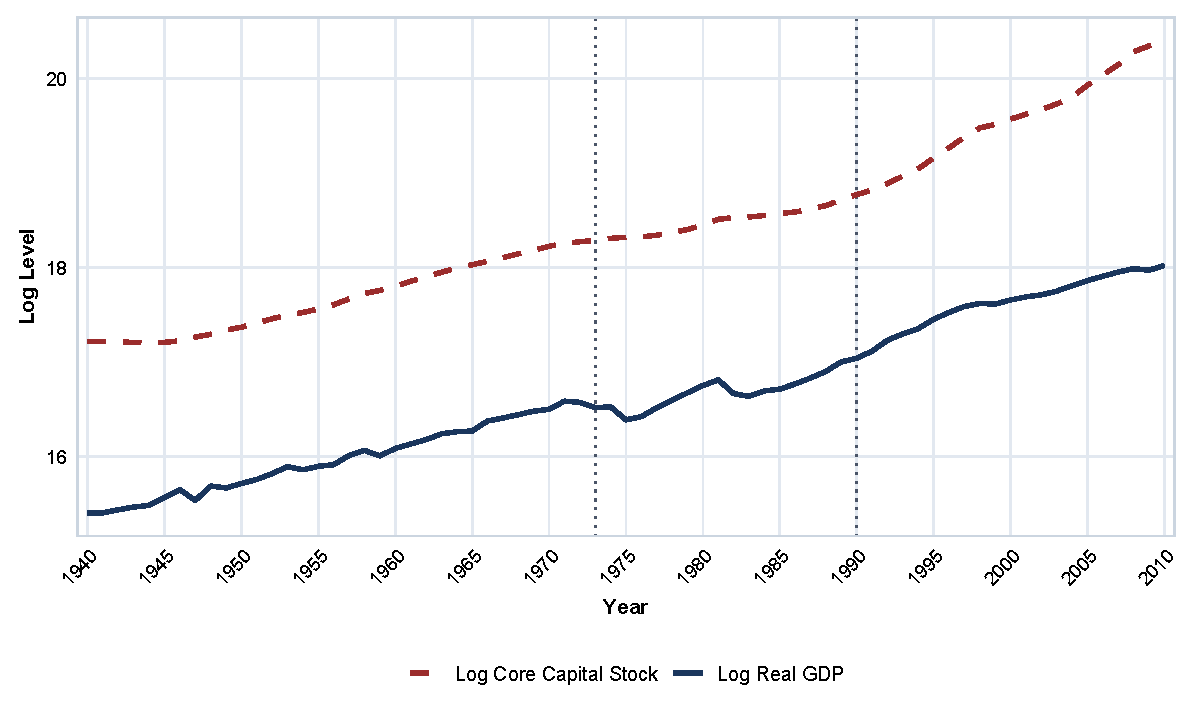
\includegraphics[width=0.92\textwidth]{figures/fig_cl_stylized_1_y_kcomponents.pdf}
\begin{singlespace}\vspace{1ex}
\multicolumn{1}{p{14.5cm}}{\footnotesize \textbf{Note:} Log real GDP ($y_t$, solid navy line), log total capital stock ($k_t^{tot}$, dashed crimson line), and log machinery and equipment ($k_t^{\text{ME}}$, dotdash green line). Vertical dotted lines mark 1973 (military coup) and 1990 (redemocratization).}
\end{singlespace}
\end{figure}
\FloatBarrier

\paragraph{H}
Figure~\ref{fig:cl_stylized_2_kappa_mechanization} plots the Chilean capital composition / mechanization gap $\kappa_t = k_t^{\text{ME}} - k_t^{\text{NRC}}$. The mechanization gap captures structural shifts in peripheral capital intensity: expanding steadily during state-led ISI (1940--1972), collapsing during early neoliberal trade liberalization and shock therapy (1973--1983), and recovering strongly during modern export-oriented resource extraction (1990--2010). This dynamic confirms the necessity of Specification B, which explicitly models the heterogeneous transformation parameter $\theta(\kappa_t)$.

\FloatBarrier
\begin{figure}[H]
\centering
\caption{Chilean Capital Composition and Mechanization Gap ($\kappa_t = k_t^{\text{ME}} - k_t^{\text{NRC}}$)}
\label{fig:cl_stylized_2_kappa_mechanization}
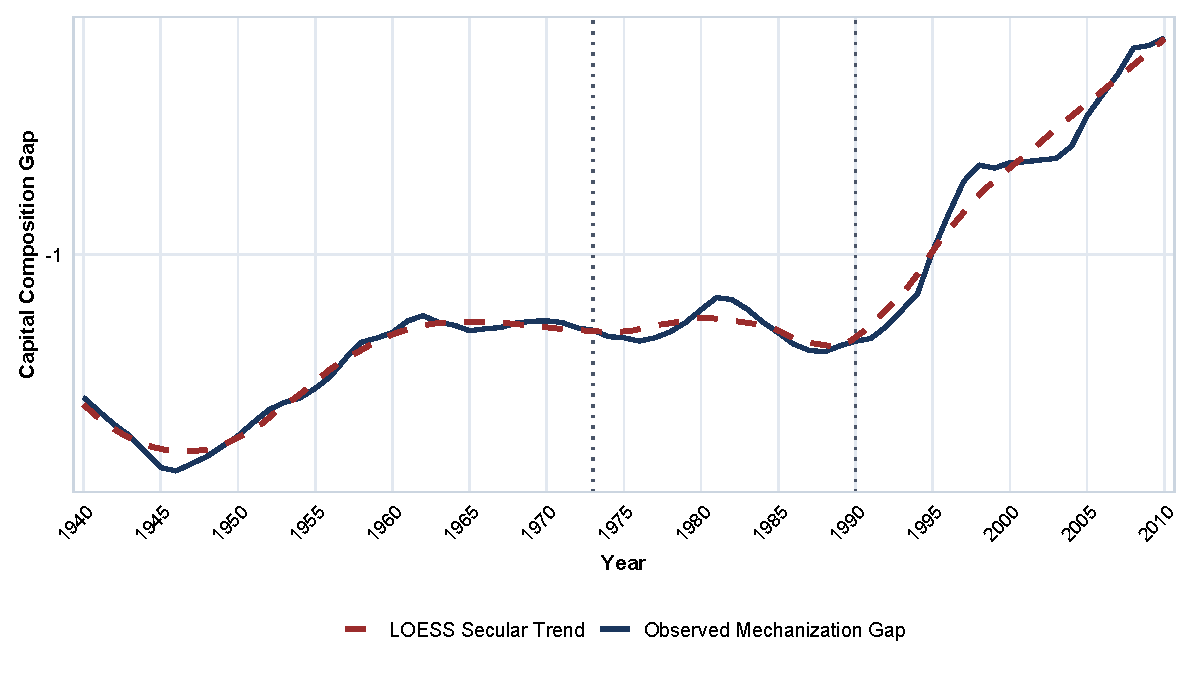
\includegraphics[width=0.92\textwidth]{figures/fig_cl_stylized_2_kappa_mechanization.pdf}
\begin{singlespace}\vspace{1ex}
\multicolumn{1}{p{14.5cm}}{\footnotesize \textbf{Note:} Observed capital composition gap $\kappa_t = k_t^{\text{ME}} - k_t^{\text{NRC}}$ (solid navy line) alongside LOESS non-parametric secular trend (dashed crimson line). Vertical lines highlight structural political shifts in 1973 and 1990.}
\end{singlespace}
\end{figure}
\FloatBarrier

\paragraph{I}
Figures~\ref{fig:cl_stylized_3_wage_share} and \ref{fig:cl_stylized_4_minipages} document the domestic distributive and external structural constraints binding peripheral capital accumulation. Figure~\ref{fig:cl_stylized_3_wage_share} displays gross and net wage share compression following the 1973 shock. Figure~\ref{fig:cl_stylized_4_minipages} disaggregates the raw physical and financial constituent series driving external realization bottlenecks: Panel 4a plots Central Bank foreign reserve solvency ($S_t$); Panel 4b plots log terms of trade ($\ln \text{ToT}_t$); Panel 4c plots log real export volume ($\ln X_t$); and Panel 4d plots log gross machinery investment ($\ln I_t^{\text{ME}}$).

\FloatBarrier
\begin{figure}[H]
\centering
\caption{Chilean Wage Share Trajectories ($\omega_t^{\text{gross}}$ and $\omega_t^{\text{net}}$)}
\label{fig:cl_stylized_3_wage_share}
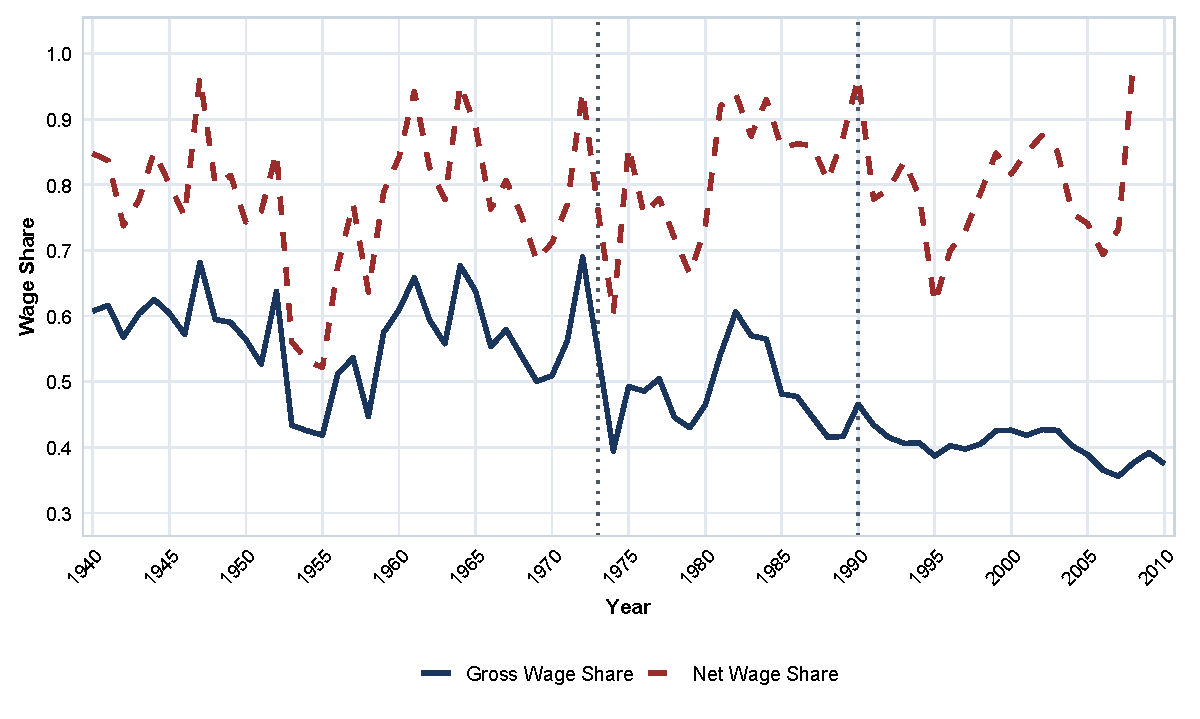
\includegraphics[width=0.92\textwidth]{figures/fig_cl_stylized_3_wage_share.pdf}
\begin{singlespace}\vspace{1ex}
\multicolumn{1}{p{14.5cm}}{\footnotesize \textbf{Note:} Gross wage share $\omega_t^{\text{gross}}$ (solid navy line) and net wage share $\omega_t^{\text{net}}$ (dashed crimson line) from 1940 to 2010.}
\end{singlespace}
\end{figure}
\FloatBarrier

\FloatBarrier
\begin{figure}[H]
\centering
\caption{Chilean External Bottleneck Constituent Series (1940--2010)}
\label{fig:cl_stylized_4_minipages}
\begin{minipage}{0.48\textwidth}
  \centering
  \textbf{(a) Central Bank Solvency Ratio ($S_t$)}\\
  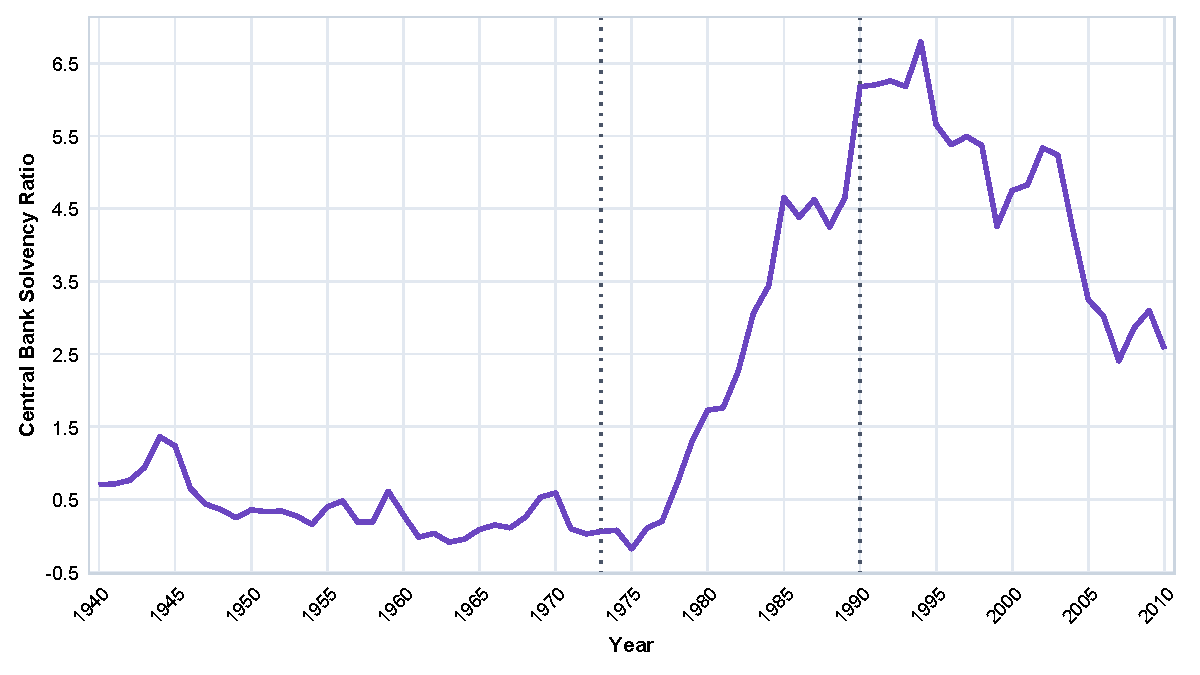
\includegraphics[width=\linewidth]{figures/fig_cl_stylized_4a_external_constraint.pdf}
\end{minipage}\hfill
\begin{minipage}{0.48\textwidth}
  \centering
  \textbf{(b) Log Terms of Trade ($\ln \text{ToT}_t$)}\\
  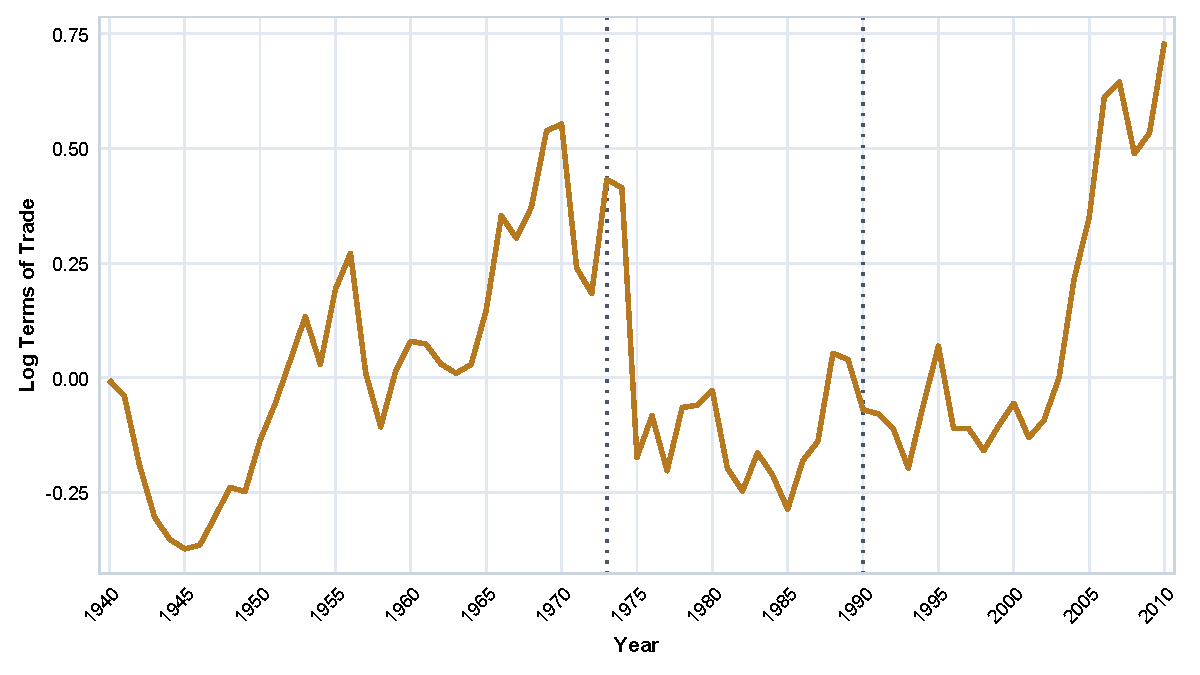
\includegraphics[width=\linewidth]{figures/fig_cl_stylized_4b_external_constraint.pdf}
\end{minipage}

\vspace{2ex}

\begin{minipage}{0.48\textwidth}
  \centering
  \textbf{(c) Log Real Exports ($\ln X_{\text{FOB},t}$)}\\
  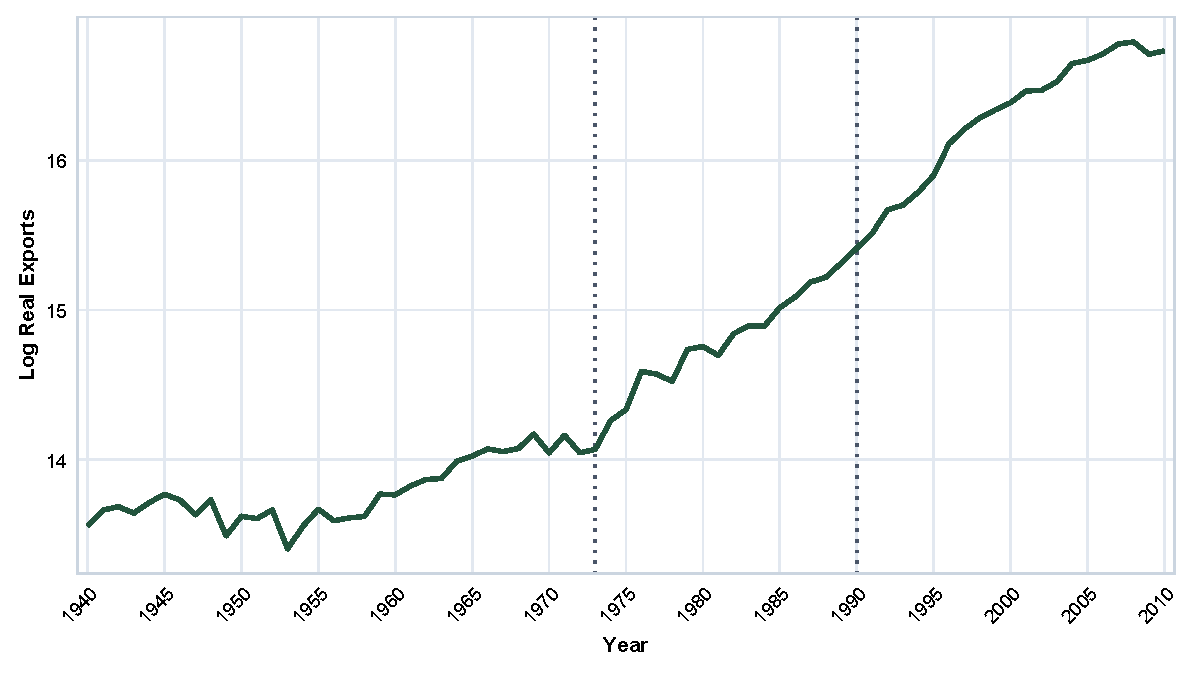
\includegraphics[width=\linewidth]{figures/fig_cl_stylized_4c_external_constraint.pdf}
\end{minipage}\hfill
\begin{minipage}{0.48\textwidth}
  \centering
  \textbf{(d) Log Machinery Investment ($\ln I_t^{\text{ME}}$)}\\
  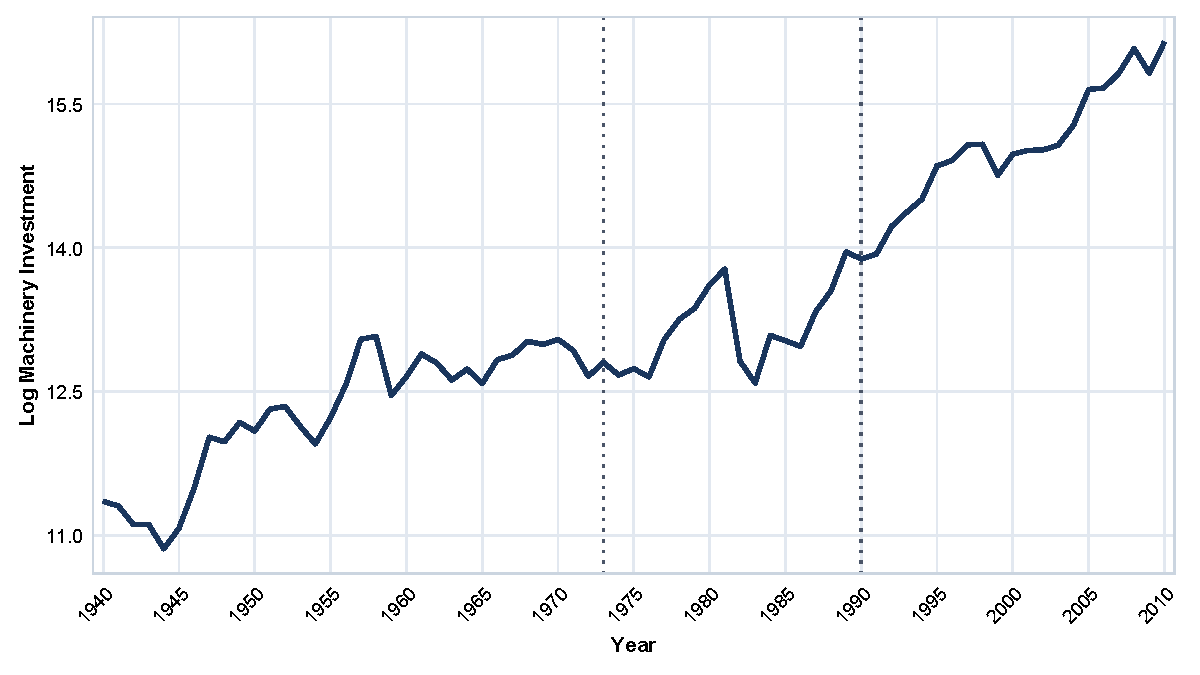
\includegraphics[width=\linewidth]{figures/fig_cl_stylized_4d_external_constraint.pdf}
\end{minipage}

\begin{singlespace}\vspace{1ex}
\multicolumn{1}{p{14.5cm}}{\footnotesize \textbf{Note:} Disaggregated empirical constituent series forming the peripheral balance-of-payments constraint. Panel (a) plots Central Bank foreign exchange reserve solvency ($S_t$). Panels (b) and (c) plot the log terms of trade and log real exports, which together compose log real capital import purchasing power ($\ln M_t^{\text{cap,ToT}} = \ln \text{ToT}_t + \ln X_t$). Panel (d) plots active gross machinery investment demand ($\ln I_t^{\text{ME}}$).}
\end{singlespace}
\end{figure}
\FloatBarrier

\begin{table}[H]
\centering
\footnotesize
\caption{Chile Descriptive Statistics (1940--2010)}
\label{tab:cl_stylized_facts_summary}
\begin{tabular}{p{7.5cm} p{2.5cm} p{2.5cm}}
\hline\hline
\textbf{Variable} & \textbf{Mean} & \textbf{Std. Dev.} \\
\hline
Log Real GDP ($y_t$) & 16.625 & 0.776 \\
Log Core Capital Stock ($k_t^{cap}$) & 18.419 & 0.899 \\
Log Output--Capital Ratio ($y_t - k_t^{cap}$) & -1.793 & 0.169 \\
Capital Composition Gap ($\kappa_t$) & -1.106 & 0.211 \\
Gross Wage Share ($\omega_t^{gross}$) & 0.501 & 0.092 \\
Net Wage Share ($\omega_t^{net}$) & 0.802 & 0.121 \\
Central Bank Solvency Ratio ($S_t$) & 2.102 & 2.201 \\
Log Terms of Trade ($\ln \text{ToT}_t$) & 0.030 & 0.263 \\
Log Real Exports ($\ln X_{\text{FOB},t}$) & 14.753 & 1.116 \\
Log Machinery Investment ($\ln I_t^{\text{ME}}$) & 13.307 & 1.335 \\
\hline\hline
\multicolumn{3}{p{12.5cm}}{\scriptsize \textbf{Note:} Sample window spans 1940--2010 ($N = 71$). Real GDP and capital stock components sourced from Díaz, Lüders and Wagner (2016) and Pérez and Eyzaguirre (2021). Core capital stock is $K_t^{cap} = K_t^{\text{ME}} + K_t^{\text{NRC}}$. Capital composition gap $\kappa_t = k_t^{\text{ME}} - k_t^{\text{NRC}}$. Both Gross wage share (nominal compensation / nominal GDP) and Net wage share (nominal compensation / nominal NVA) are evaluated in nominal terms. Structural threshold $\hat{\gamma} = 0.425$ separates binding foreign exchange bottleneck regimes.} \\
\end{tabular}
\end{table}


